% Created 2021-09-11 Sat 09:35
% Intended LaTeX compiler: xelatex
\documentclass[letterpaper]{article}
\usepackage{graphicx}
\usepackage{grffile}
\usepackage{longtable}
\usepackage{wrapfig}
\usepackage{rotating}
\usepackage[normalem]{ulem}
\usepackage{amsmath}
\usepackage{textcomp}
\usepackage{amssymb}
\usepackage{capt-of}
\usepackage{hyperref}
\usepackage[margin=1in]{geometry}
\usepackage{fontspec}
\usepackage{indentfirst}
\setmainfont[ItalicFont = LiberationSans-Italic, BoldFont = LiberationSans-Bold, BoldItalicFont = LiberationSans-BoldItalic]{LiberationSans}
\newfontfamily\NHLight[ItalicFont = LiberationSansNarrow-Italic, BoldFont       = LiberationSansNarrow-Bold, BoldItalicFont = LiberationSansNarrow-BoldItalic]{LiberationSansNarrow}
\newcommand\textrmlf[1]{{\NHLight#1}}
\newcommand\textitlf[1]{{\NHLight\itshape#1}}
\let\textbflf\textrm
\newcommand\textulf[1]{{\NHLight\bfseries#1}}
\newcommand\textuitlf[1]{{\NHLight\bfseries\itshape#1}}
\usepackage{fancyhdr}
\pagestyle{fancy}
\usepackage{titlesec}
\usepackage{titling}
\makeatletter
\lhead{\textbf{\@title}}
\makeatother
\rhead{\textrmlf{Compiled} \today}
\lfoot{\theauthor\ \textbullet \ \textbf{2021-2022}}
\cfoot{}
\rfoot{\textrmlf{Page} \thepage}
\titleformat{\section} {\Large} {\textrmlf{\thesection} {|}} {0.3em} {\textbf}
\titleformat{\subsection} {\large} {\textrmlf{\thesubsection} {|}} {0.2em} {\textbf}
\titleformat{\subsubsection} {\large} {\textrmlf{\thesubsubsection} {|}} {0.1em} {\textbf}
\setlength{\parskip}{0.45em}
\renewcommand\maketitle{}
\author{Houjun Liu}
\date{\today}
\title{Enzymes}
\hypersetup{
 pdfauthor={Houjun Liu},
 pdftitle={Enzymes},
 pdfkeywords={},
 pdfsubject={},
 pdfcreator={Emacs 27.2 (Org mode 9.4.4)}, 
 pdflang={English}}
\begin{document}

\maketitle


\section{Enzymes}
\label{sec:org33f5e15}
Proteins that build things up and break things down!

\begin{quote}
*Enzymes are catalysts. They speed reaction rates but do not affect
the change in free energy of the reaction (the difference in potential
energy between reactants and products).*
\end{quote}

A macromolecular \textbf{catalyst}, it\ldots{}

\begin{enumerate}
\item Speeds up the rate of reactions
\item Does not get consumed by the reaction

\begin{enumerate}
\item Not a fundimental product
\item Not a fundiment reactant
\end{enumerate}

\item Shape determines the reactions that it can participate in
\item Enzymes are subject to \textbf{protean denaturation} => if the protein
unfolds, its function will be lost. Triggered by excess heat, acid,
and other problems

\item is unlike non-protein, inorganic catalyst --- inorganic non-proteins
need to unwrap or wrap.
\end{enumerate}

\begin{figure}[htbp]
\centering
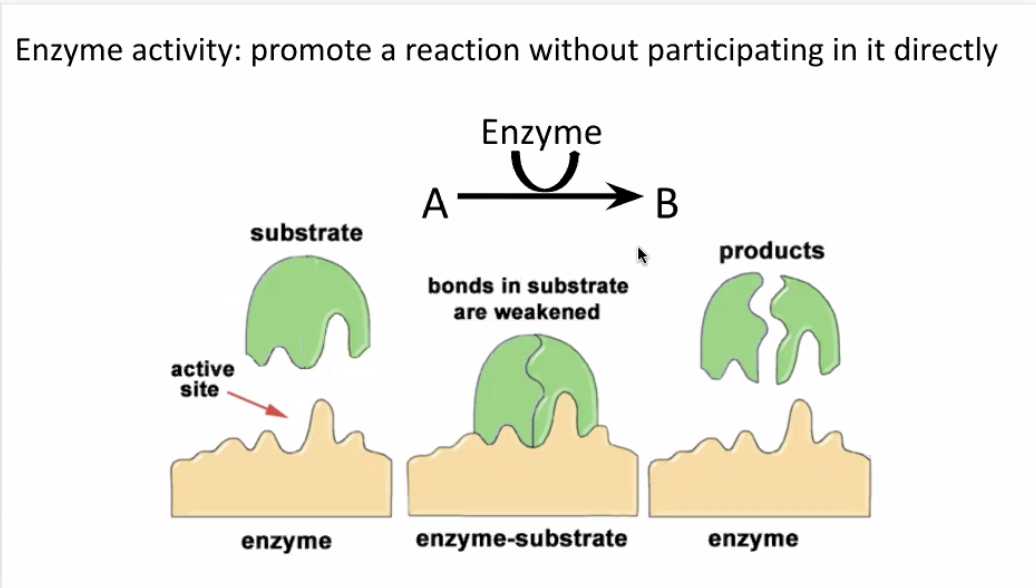
\includegraphics[width=.9\linewidth]{Screen Shot 2020-09-30 at 2.45.04 PM.png}
\caption{Screen Shot 2020-09-30 at 2.45.04 PM.png}
\end{figure}

\subsection{Enzymes doing things}
\label{sec:orgbc19cff}
\begin{enumerate}
\item The reactant (called "substrate") fits into a pocket ("active site")
in the enzyme for the reaction to occur. Yes, there could be multiple
active sites for multiple reactants
\item The enzyme rearrange itself slightly to hold the enzyme in place.
This is called "induced fit"
\item A cofactor ("catalyst to the catalyst") also bind to the active sites
\end{enumerate}

Enzymes minimize the \textbf{activation energy hump}

\subsection{Why do Enzymes work?}
\label{sec:org37ee96e}
There are three main ways that Enzymes work:

\begin{enumerate}
\item Stress and straining of the bonds to force towards the nessariy
transition state
\item Changing the substrate to gavourable orientation
\item Active site animo acids rearranging electrons + creating partial
charges to favor a reaction
\end{enumerate}

Or, in Dr. Hauser's Words

““” - Orienting the reactions substrate(s) to promote more effective
collisions (and therefore reactions - Stressing or straining bonds to
temporarily and/or slightly lower the strength of attraction to allow
the bond to break more easily - Involving amino acid R-groups or
sidechains in creating the transition state between reactants and
products ““”

\textbf{Remember: The Fundamental Energy Difference does not change whether or
not reactions are helped by the Enzyme.}

For more information about the reaction hump and its related energy
changes, see \href{KBhBIO101Enthalpy.org}{KBhBIO101Enthalpy}, and
\href{KBhBIO101Entropy.org}{KBhBIO101Entropy}.

If the body needs a favorable reaction, Enzymes make them quicker. If
the body needs a non-favorable reaction, Enzymes catches the energy to
make it happen.
\end{document}
